\documentclass[border=10pt]{standalone}
\usepackage[svgnames]{xcolor}
\usepackage{amsmath}
\usepackage{pgfplots}
\pgfplotsset{compat=newest}
\usepackage[sfdefault]{FiraSans}
\usepackage{FiraMono}
\renewcommand*\familydefault{\sfdefault}
\begin{document}
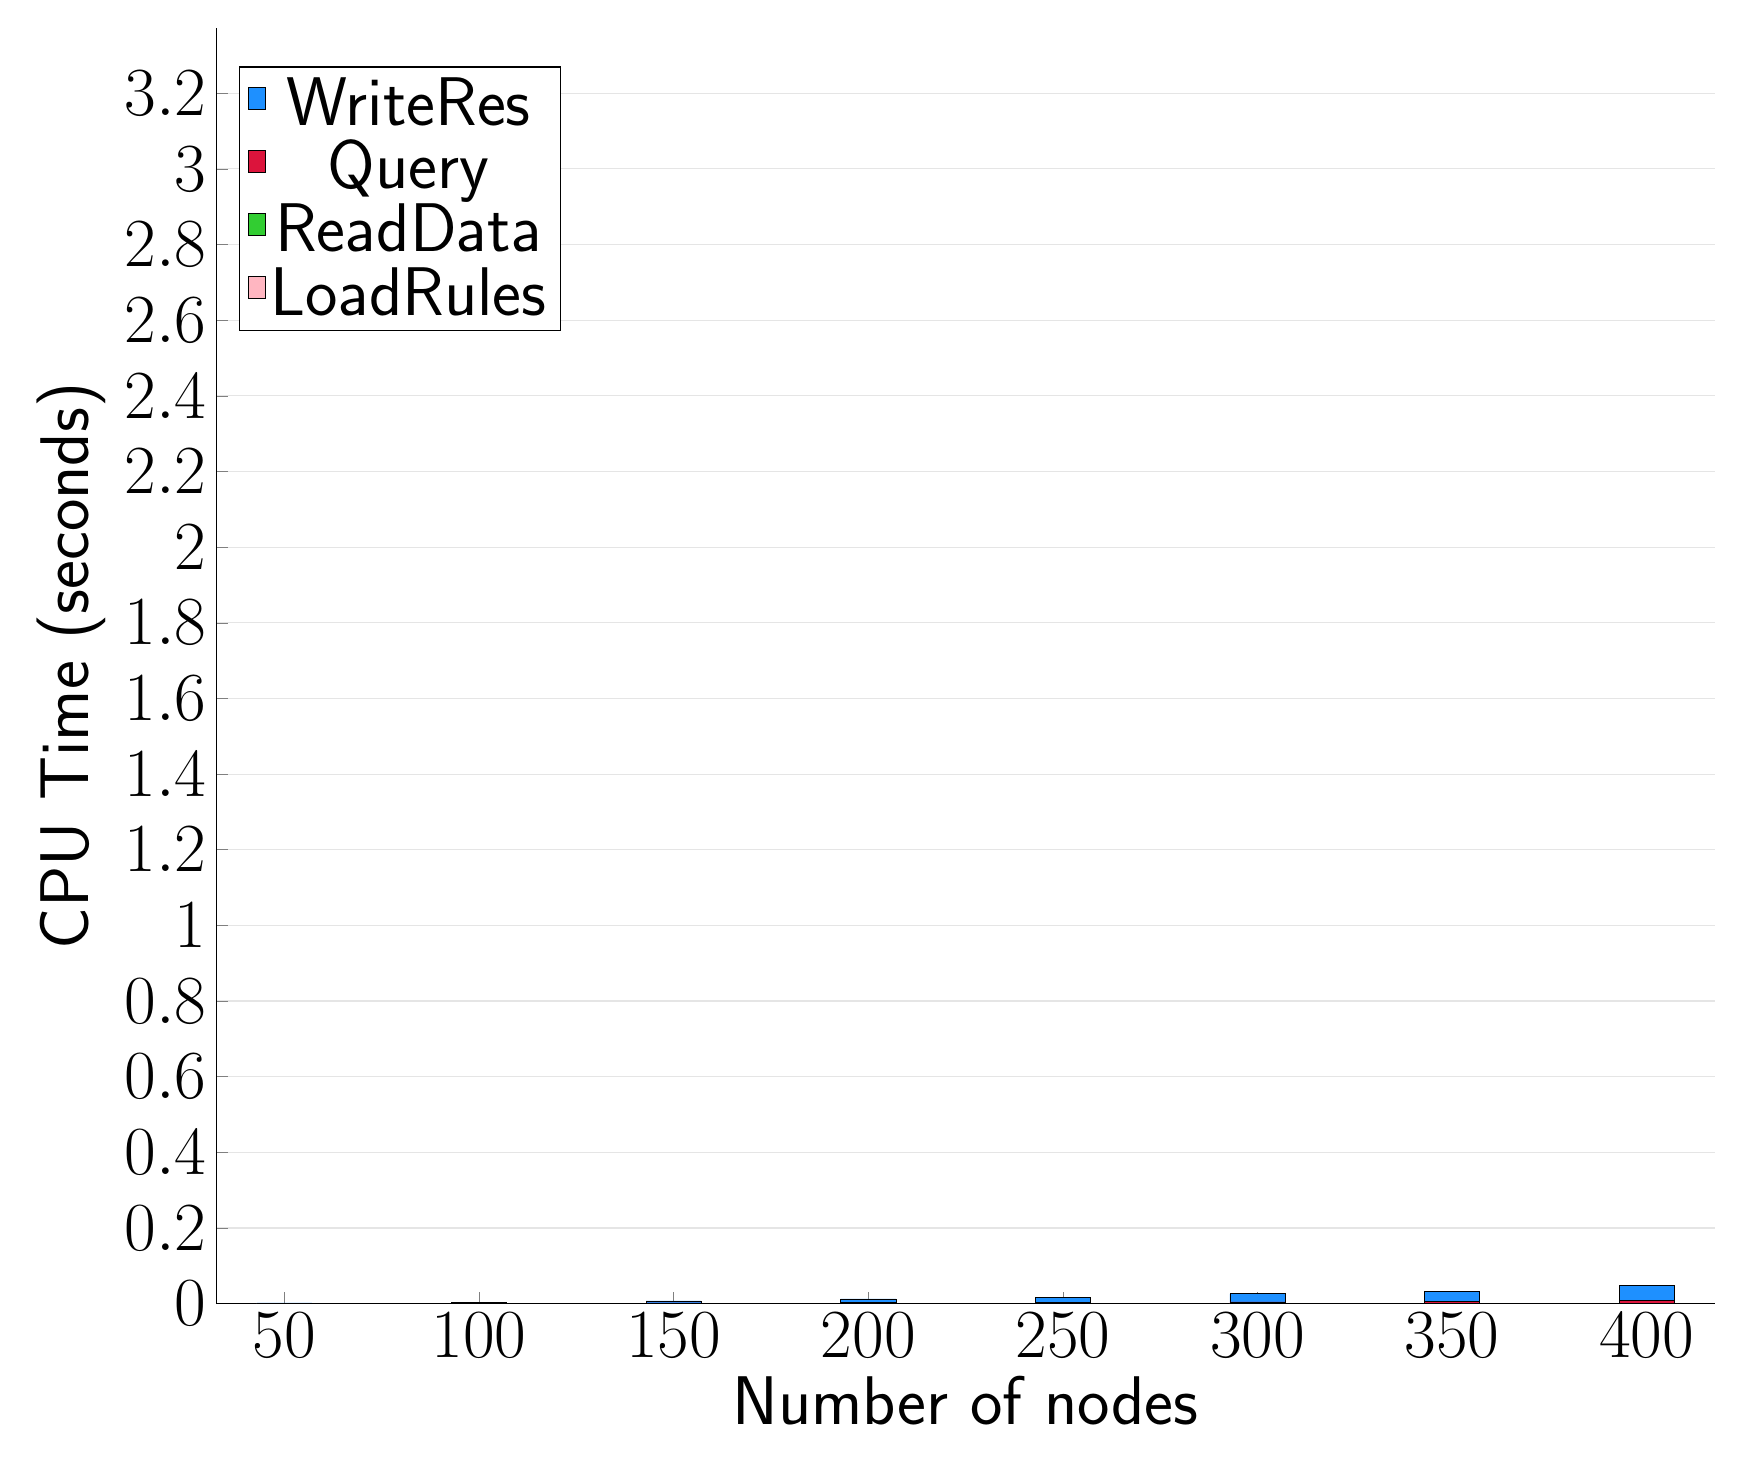
\begin{tikzpicture}
\begin{axis}[
   ybar stacked,
   width=1.7\textwidth,
   bar width=0.7cm,
   ymajorgrids, tick align=inside,
   major grid style={draw=gray!20},
   xtick=data,
   ymin=0, ymax=3.3720000000000003,
   axis x line*=bottom,
   axis y line*=left,
   enlarge x limits=0.05,
   legend style={
       at={(0.23, 0.97)},
       anchor=north east,
       legend columns=1,
       font=\Huge,
   },
   ylabel={CPU Time (seconds)},
   xlabel={Number of nodes},
   label style={font=\Huge},
   tick label style={font=\Huge},
]
\addlegendimage{fill=DodgerBlue, draw=black, line width=0.2pt}
\addlegendentry{WriteRes}
\addlegendimage{fill=Crimson, draw=black, line width=0.2pt}
\addlegendentry{Query}
\addlegendimage{fill=LimeGreen, draw=black, line width=0.2pt}
\addlegendentry{ReadData}
\addlegendimage{fill=LightPink, draw=black, line width=0.2pt}
\addlegendentry{LoadRules}
\addplot +[fill=LightPink, draw=black, line width=0.2pt] coordinates {
(50, 0.0006118999999999996)
(100, 0.0006121999999999999)
(150, 0.0006184)
(200, 0.0006035000000000004)
(250, 0.0006374000000000004)
(300, 0.0006142)
(350, 0.0006053000000000001)
(400, 0.0006104999999999998)
};
\addplot +[fill=LimeGreen, draw=black, line width=0.2pt] coordinates {
(50, 0.00021480000000000018)
(100, 0.0002908000000000001)
(150, 0.0003622)
(200, 0.0004423000000000002)
(250, 0.000511599999999999)
(300, 0.0005992)
(350, 0.0006670999999999997)
(400, 0.0007891000000000006)
};
\addplot +[fill=Crimson, draw=black, line width=0.2pt] coordinates {
(50, 0.0001294999999999996)
(100, 0.0004586999999999998)
(150, 0.0009027999999999998)
(200, 0.0016041)
(250, 0.0022034000000000003)
(300, 0.0033685)
(350, 0.0042209)
(400, 0.0064233)
};
\addplot +[fill=DodgerBlue, draw=black, line width=0.2pt] coordinates {
(50, 0.0007276000000000007)
(100, 0.0027120000000000004)
(150, 0.0055442)
(200, 0.010098300000000001)
(250, 0.013196100000000002)
(300, 0.021485499999999998)
(350, 0.026588800000000003)
(400, 0.040131299999999995)
};
\end{axis}
\end{tikzpicture}

\end{document}
